%% ----------------------------------------------------------------
%% AppendixAuthoringToolWireframes.tex
%% ---------------------------------------------------------------- 
\chapter{Authoring Tool Wireframes} \label{App:Authoring Tool Wireframes}

\begin{preamble}
	An appendix showing the initial authoring tool wireframes. These were used as examples of the interface was planned until the HTML views were created and iterated upon.
\end{preamble}

\section{Introduction}

Wireframes were created to allow for feedback from users and the client regarding potential designs for the Authoring tool. These initial wireframes were presented to Shameem for the first user evaluations to give a rough idea of what would be designed.

\section{Authoring Tool Primary User Interface}

When designing the user interface for the authoring tool there were initially had two main concepts. There were to be a large amount of settings to configure when using the tool and overloading the user was to be avoided (\cref{Req:User interface}). Therefore it was planned to hide most of the options initially.

This led to deciding on two different options for the hiding of this interface.

\subsection{First Option - Accordion} 

The first option considered was using an accordion view shown in \autoref{Figure:wireframes/authoringtool/accordion}. Here the options for each part of the question sets are shown in accordions that appear as the question set is edited.

This meant that only the options for the current question you were working on were shown but that you could switch between different questions to review the information.

\begin{figure}
	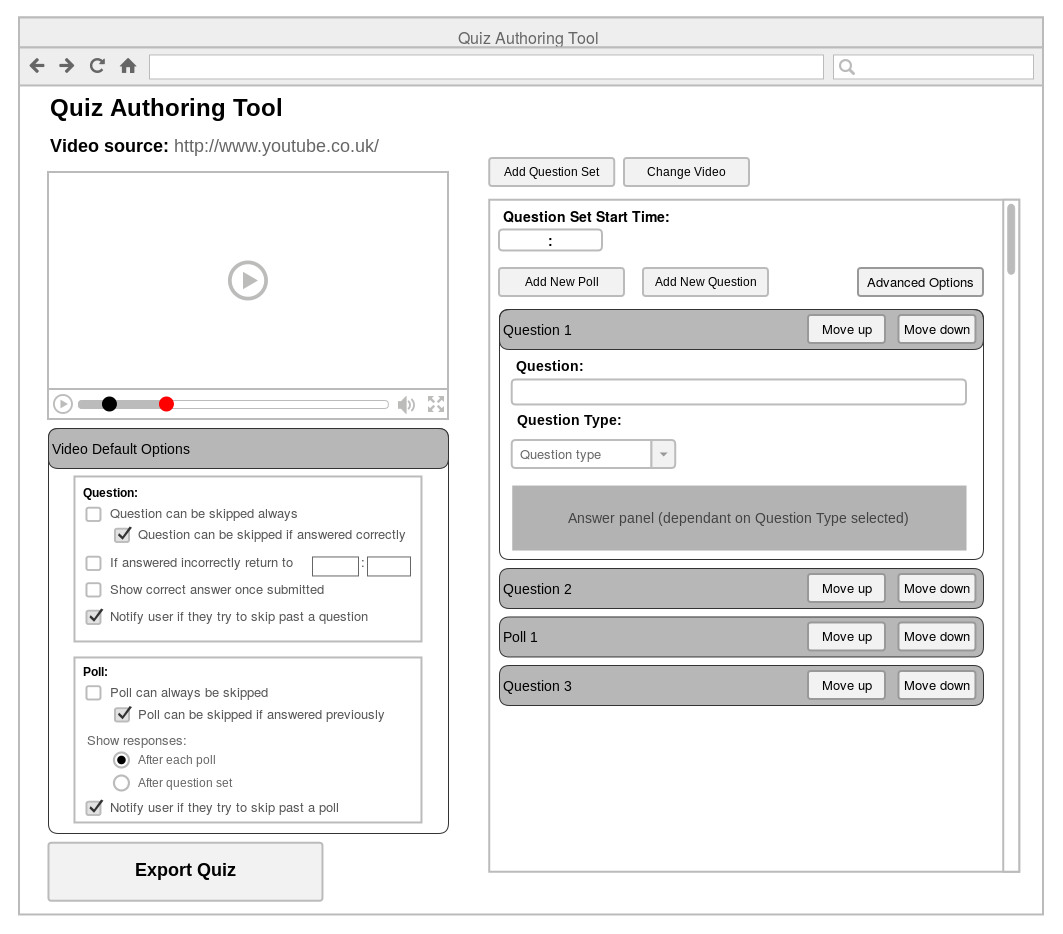
\includegraphics[width=\textwidth]{wireframes/gdpAuthoringAccordianVideoDefaultOptions.png}
	\caption{Wireframe showing the accordion type design of showing/hiding options}
	\label{Figure:wireframes/authoringtool/accordion}
\end{figure}

\subsection{Second Option - Pop ups}

A second option was considered where you would press an edit button and the options would pop up. Here you originally see the main screen shown in \autoref{Figure:wireframes/authoringtool/main} and then once you select an options button such as the ``advanced option'' button, you would see the popup shown in \autoref{Figure:wireframes/authoringtool/mainPopup}.

\begin{landscape}

\begin{figure}
	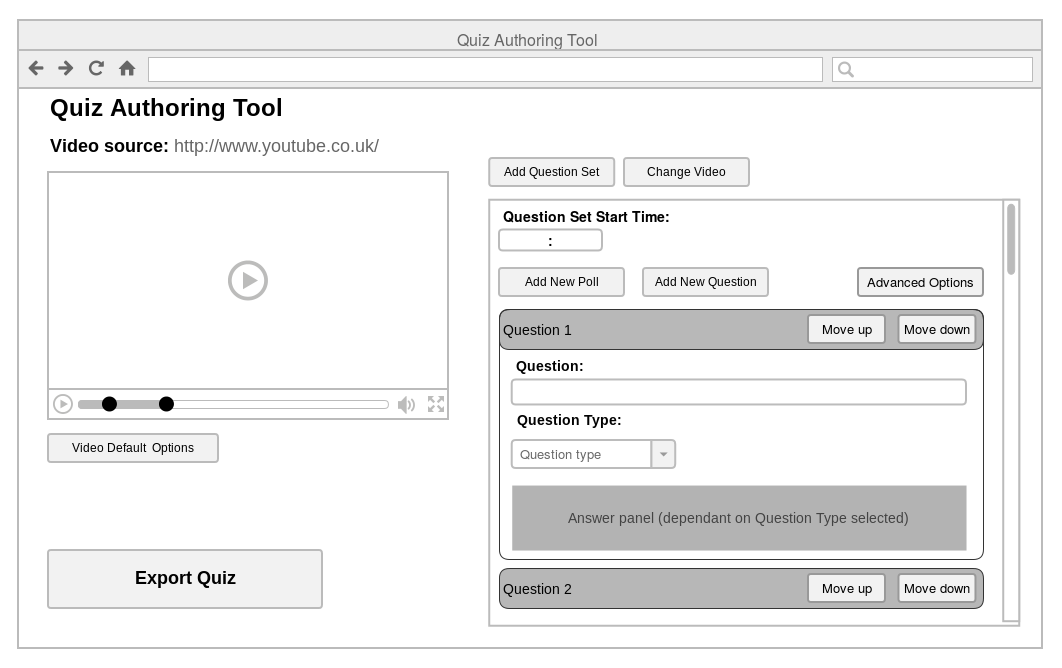
\includegraphics[width=22cm]{wireframes/gdpAuthoringMain.png}
	\caption{Wireframe showing the pop up type design of showing/hiding options before opening a pop up.}
	\label{Figure:wireframes/authoringtool/main}
\end{figure}

\begin{figure}
	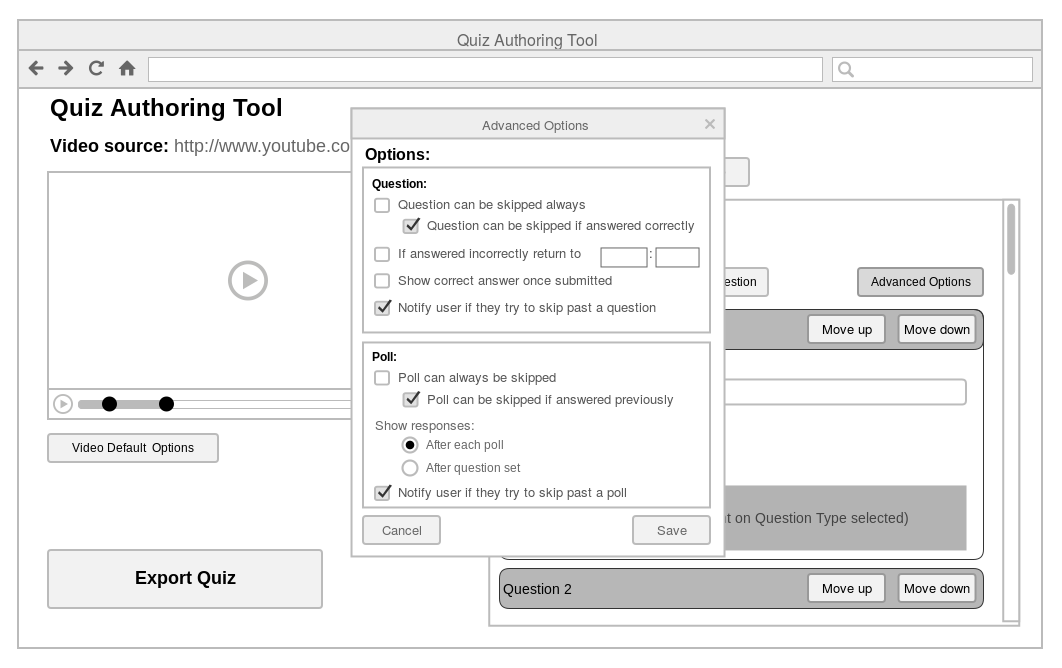
\includegraphics[width=22cm]{wireframes/gdpAuthoringAdvancedOptions.png}
	\caption{Wireframe showing the accordion type design of showing/hiding options after opening a pop up.}
	\label{Figure:wireframes/authoringtool/mainPopup}
\end{figure}
\end{landscape}


\section{Question Creation Wireframes}

These first wireframes (\autoref{Figure:wireframes/authoringtool/singlePoll}, \autoref{Figure:wireframes/authoringtool/singleQuiz}, \autoref{Figure:wireframes/authoringtool/multiPoll}, \autoref{Figure:wireframes/authoringtool/multiQuiz}, \autoref{Figure:wireframes/authoringtool/rangeStarPoll}, \autoref{Figure:wireframes/authoringtool/rangeStarQuiz}) show how the questions were originally planned to look. This demonstrates the differences between the poll and quiz type options, where the quiz type questions allow the choice of a ``correct" answer. These were used to generate the first iteration of HTML from the mockups, which were iterated over. This was because it was easier to have more realistic models to present to users and the client.

\begin{figure}
	\centering
	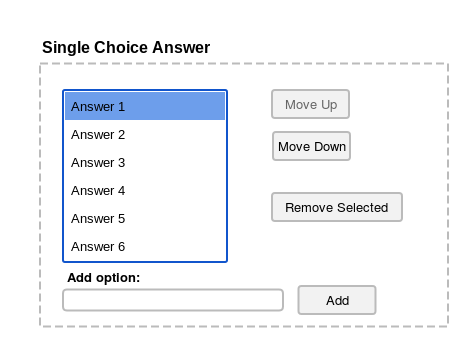
\includegraphics[width=12cm]{wireframes/gdpauthoringsingleanswerpoll.png}
	\caption{A wireframe showing the possible interface when creating a single choice poll type question}
	\label{Figure:wireframes/authoringtool/singlePoll}
\end{figure}

\begin{figure}
	\centering
	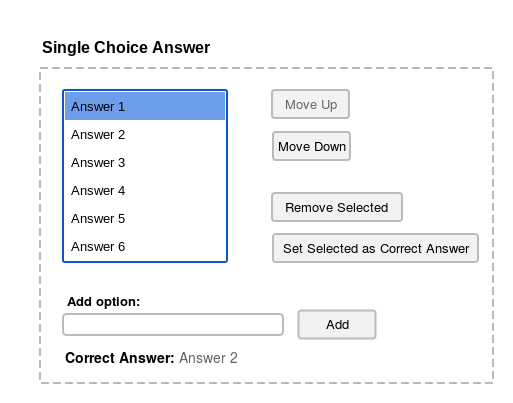
\includegraphics[width=12cm]{wireframes/gdpauthoringsingleanswerquestion.png}
	\caption{A wireframe showing the possible interface when creating a single choice quiz type question}
	\label{Figure:wireframes/authoringtool/singleQuiz}
\end{figure}

\begin{figure}
	\centering
	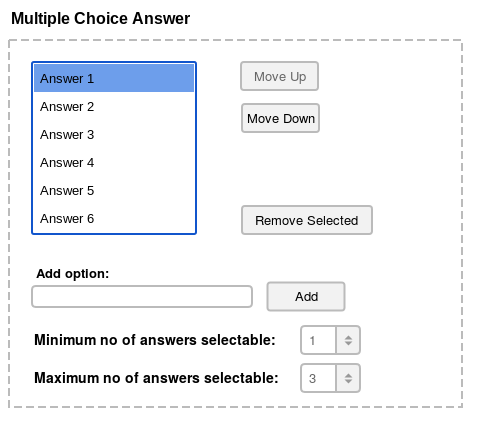
\includegraphics[width=10cm]{wireframes/gdpauthoringmultianswerpoll.png}
	\caption{A wireframe showing the possible interface when creating a multiple choice poll type question}
	\label{Figure:wireframes/authoringtool/multiPoll}
\end{figure}

\begin{figure}
	\centering
	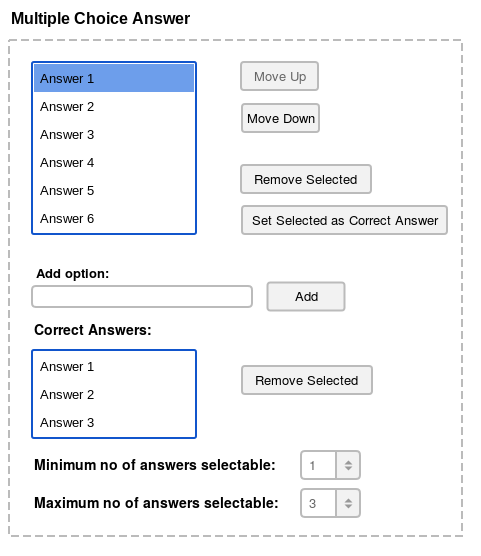
\includegraphics[width=10cm]{wireframes/gdpauthoringmultianswerquestion.png}
	\caption{A wireframe showing the possible interface when creating a multiple choice quiz type question}
	\label{Figure:wireframes/authoringtool/multiQuiz}
\end{figure}

\begin{figure}
	\centering
	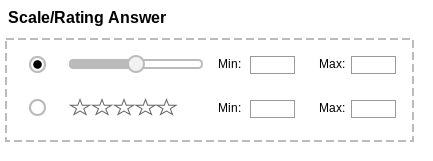
\includegraphics[width=10cm]{wireframes/gdpauthoringscalepoll.png}
	\caption{A wireframe showing the possible interface when creating a range or star poll type question}
	\label{Figure:wireframes/authoringtool/rangeStarPoll}
\end{figure}


\begin{figure}
	\centering
	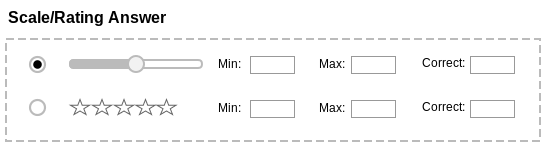
\includegraphics[width=12cm]{wireframes/gdpauthoringscalequestion.png}
	\caption{A wireframe showing the possible interface when creating a range or star quiz type question}
	\label{Figure:wireframes/authoringtool/rangeStarQuiz}
\end{figure}

\section{Accessibility Tooltips}

To aid accessibility the appearance tooltips on some elements was planned. This was illustrated in the example tooltip wireframe \autoref{Figure:wireframes/authoringtool/tooltip}.

\begin{landscape}
\begin{figure}
	\centering
	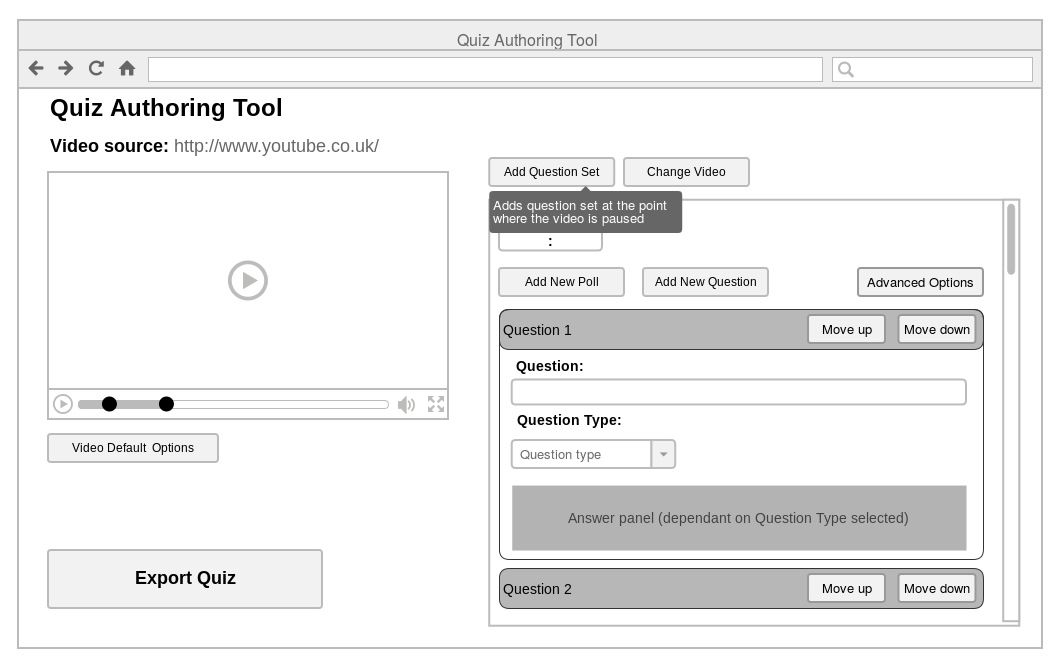
\includegraphics[width=22cm]{wireframes/gdpAuthoringToolTip.png}
	\caption{A wireframe showing an example of how tooltips could be implemented}
	\label{Figure:wireframes/authoringtool/tooltip}
\end{figure}
\end{landscape}